\documentclass[slovene,11pt,a4paper]{article}
\usepackage[pdftex]{graphicx}
\DeclareGraphicsExtensions{.pdf,.png}


\usepackage{tikz}
\usepackage{float}
\usepackage[margin=2cm,bottom=3cm,foot=1.5cm]{geometry}
\usepackage{fullpage}
\usepackage{a4wide}
\setlength{\parindent}{0pt}
\setlength{\parskip}{0.5ex}
\usepackage{amsmath}
\usepackage{amsfonts}
\usepackage{mathrsfs}
\usepackage[usenames]{color}
\usepackage[utf8]{inputenc}
\usepackage{siunitx}
\usepackage{caption}

\DeclareCaptionType{equ}[][]
\def\phi{\varphi}
\def\eps{\varepsilon}
\def\theta{\vartheta}

\newcommand{\thisyear}{2020/21}

\renewcommand{\Re}{\mathop{\rm Re}\nolimits}
\renewcommand{\Im}{\mathop{\rm Im}\nolimits}
\newcommand{\Tr}{\mathop{\rm Tr}\nolimits}
\newcommand{\diag}{\mathop{\rm diag}\nolimits}
\newcommand{\dd}{\,\mathrm{d}}
\newcommand{\ddd}{\mathrm{d}}
\newcommand{\ii}{\mathrm{i}}
\newcommand{\lag}{\mathcal{L}\!}
\newcommand{\ham}{\mathcal{H}\!}
\newcommand{\four}[1]{\mathcal{F}\!\left(#1\right)}
\newcommand{\bigO}[1]{\mathcal{O}\!\left(#1\right)}
\newcommand{\sh}{\mathop{\rm sinh}\nolimits}
\newcommand{\ch}{\mathop{\rm cosh}\nolimits}
\renewcommand{\th}{\mathop{\rm tanh}\nolimits}
\newcommand{\erf}{\mathop{\rm erf}\nolimits}
\newcommand{\erfc}{\mathop{\rm erfc}\nolimits}
\newcommand{\sinc}{\mathop{\rm sinc}\nolimits}
\newcommand{\rect}{\mathop{\rm rect}\nolimits}
\newcommand{\ee}[1]{\cdot 10^{#1}}
\newcommand{\inv}[1]{\left(#1\right)^{-1}}
\newcommand{\invf}[1]{\frac{1}{#1}}
\newcommand{\sqr}[1]{\left(#1\right)^2}
\newcommand{\half}{\frac{1}{2}}
\newcommand{\thalf}{\tfrac{1}{2}}
\newcommand{\pd}{\partial}
\newcommand{\Dd}[3][{}]{\frac{\ddd^{#1} #2}{\ddd #3^{#1}}}
\newcommand{\Pd}[3][{}]{\frac{\pd^{#1} #2}{\pd #3^{#1}}}
\newcommand{\avg}[1]{\left\langle#1\right\rangle}
\newcommand{\norm}[1]{\left\Vert #1 \right\Vert}
\newcommand{\braket}[2]{\left\langle #1 \vert#2 \right\rangle}
\newcommand{\obraket}[3]{\left\langle #1 \vert #2 \vert #3 \right \rangle}
\newcommand{\hex}[1]{\texttt{0x#1}}

\renewcommand{\iint}{\mathop{\int\mkern-13mu\int}}
\renewcommand{\iiint}{\mathop{\int\mkern-13mu\int\mkern-13mu\int}}
\newcommand{\oiint}{\mathop{{\int\mkern-15mu\int}\mkern-21mu\raisebox{0.3ex}{$\bigcirc$}}}

\newcommand{\wunderbrace}[2]{\vphantom{#1}\smash{\underbrace{#1}_{#2}}}

\renewcommand{\vec}[1]{\overset{\smash{\hbox{\raise -0.42ex\hbox{$\scriptscriptstyle\rightharpoonup$}}}}{#1}}
\newcommand{\bec}[1]{\mathbf{#1}}




\newcommand{\Ai}{\mathrm{Ai}}
\newcommand{\Bi}{\mathrm{Bi}}
\newcommand{\bi}[1]{\hbox{\boldmath{$#1$}}}
\newcommand{\bm}[1]{\hbox{\underline{$#1$}}}

\title{1. Izračun Airyjevih funkcij}
\author{Matic Tonin - 28181098 }
\date{Oktober 2020}


\usepackage[style=numeric,backend=biber,sorting=none]{biblatex}
%\usepackage{float}
\addbibresource{Viri.bib}
\sisetup{separate-uncertainty = true,multi-part-units=single}
\sisetup{output-decimal-marker = {,}}

\begin{document}

\begin{center}
\thispagestyle{empty}
\parskip=14pt%
\vspace*{3\parskip}%
\begin{Huge}Robni pogoji transportne in difuzijske enačbe\end{Huge}


Seminar v sklopu predmeta \\
Fizika nevtronskih jedrskih naprav

Avtor:

Matic Tonin

Vpisna številka: 28181098


Profesor: Izredni profesor dr. Luka Snoj 

Asistent: Andrej Žohar

\rule{7cm}{0.4pt}

Pod okvirom:

FAKULTETE ZA FIZIKO IN MATEMATIKO, LJUBLJANA

Akademsko leto 2021/2022


\end{center}
\pagebreak

\section{Uvod}
Difuzijska enačba in transportna enačba sta dve izmed osnovnih enačb za napovedovanje gibanja snovi v prostoru. V fiziki opisujeta makroskopsko gibanje mikroskopskih delcev, ki se gibljejo po principu Brownovega gibanja \footnote{Brownovo gibanje je naključno gibanje delca v določenem mediju (plin ali tekočina).}, kar povzroči naključne trke in premike. V teh dveh enačbah pa gibanje delcev ne obravnavamo posamično, ampak se osredotočamo na dve glavni količini; gostoto $\rho$ in tok $\vec{j}$. \\ 
V jedrski fiziki je tako glavni cilj opisati gibanje nevtronov v sredici jedrskega reaktorja, pri čemer moramo upoštevati tudi trke med nevtroni in jedri, ki se nahajajo v sredici. Zato definirajmo nekaj količin, ki nam bodo pomagale pri računanju.
\begin{table}[H]
\centering
 \begin{tabular}{|c| c| } 
 \hline
 Količina & Opis in Oznaka  \\ [0.5ex] 
 \hline\hline
 Številska gostota nevtronov. & Pove št nevtronov v volumnu $N(r,t)$   \\ 
 Makroskopski presek za reakcijo & Presek za reakcijo $\sum$    \\
 Število reakcij na volumsko enoto & $F(r,t)$=v\sum N(r,t)   \\
 Nevtronski fluks & $\psi(r,t)=v\sum$  \\
  Kotna nevtronska gostota & $(r,E,\vec{\Omega},t)\text{d}r^3\text{d}E\text{d}\vec{\Omega}$  \\  
    Kotni nevtronski fluks & $\phi(r,E,\vec{\Omega},t)$  \\ 
    Kotni nevtronski fluks & $\phi(r,E,\vec{\Omega},t)$   \\ 
    Kotna gostota nevtronskega toka & $j(r,E,\vec{\Omega},t)$   \\ 
    Kotno število reakcij na volumsko enoto & $f(r,t)=v\sum n(r,t)$  \\
    Gostota nevtronskega toka & $J(r,E,t)=\int \text{d}\Omega j(r,E,\vec{\Omega},t))$ \\
 \hline
 \end{tabular}
 \caption{Tabela količin, ki so uporabljene v transportni in difuzijski enačbi}
\end{table}
Iz danih kotnih količin lahko nato definiramo kotni volumen, iz katerega bodo odhajali in prihajali elektroni. Ta se bo spreminjal z enačbo \eqref{Angular_volume}. 
\begin{equation}
\left[\int_{V} \frac{\partial n}{\partial t} d^{3} r\right] d E d \hat{\Omega}=\text {pritok } V-\text {odtok } V
\label{Angular_volume}
\end{equation}
Sedaj bomo klasificirali različne načine, kako lahko elektroni pridejo in odidejo iz snovi.
\begin{enumerate}
    \item Pritoki elektronov
    \begin{itemize}
        \item Izvori nevtronov
        \item Pritoki skozi površino voluma
        \item Nevtroni drugačni energij, ki zaradi trkov preidejo v energijo $E$
    \end{itemize}
    \item Izgube elektronov
    \begin{itemize}
        \item Odtoki nevtronov skozi površino S
        \item Trki nevtronov in absorbcija elektronov v jedrih
    \end{itemize}
\end{enumerate}
Če bi sestavili vse člene skupaj, bi na koncu dobili \textbf{transportno enačbo}
\begin{equation}
\begin{aligned}
&\frac{\partial n}{\partial t}+\boldsymbol{v} \hat{\boldsymbol{\Omega}} \cdot \boldsymbol{\nabla} n+v \boldsymbol{\Sigma}, n(\mathbf{r}, \boldsymbol{E}, \hat{\boldsymbol{\Omega}}, t) \\
&\quad=\int_{4 \pi} d \hat{\boldsymbol{\Omega}}^{\prime} \int_{0}^{\infty} d E^{\prime} v^{\prime} \Sigma_{\mathbf{s}}\left(E^{\prime} \rightarrow E, \hat{\boldsymbol{\Omega}}^{\prime} \rightarrow \hat{\boldsymbol{\Omega}}\right) n\left(\mathbf{r}, E^{\prime}, \hat{\boldsymbol{\Omega}}^{\prime}, t\right)+s(\mathbf{r}, E, \hat{\boldsymbol{\Omega}}, t)
\end{aligned},
\label{Transportna enačba}
\end{equation}
ki je oblike lineare enačbe s parametri $n(\vec{r}(x,y,z),E,\Omega(\theta,\phi), t)$, zaradi vsebovanja obeh odvodov (časovnega in krajevnega) in integracije po energijah in kotu pa jo uvrščamo med integralnodiferencialne enačbe.

V primeru, ko bi našo transportnpo enačbo \eqref{Transportna enačba} integrirali po prostorskem kotu, bi tako prešli iz številske gostote elektronov na tok elektronov in dobili novo enačbo \begin{equation}
\frac{1}{v} \frac{\partial \phi}{\partial t}+\nabla \cdot \mathbf{J}(\mathbf{r}, E, t)+\Sigma_{t}(\mathbf{r}, E) \phi(\mathbf{r}, E, t)=\int_{0}^{\infty} d E^{\prime} \Sigma_{s}\left(E^{\prime} \rightarrow E\right) \phi\left(\mathbf{r}, E^{\prime}, t\right)+S(\mathbf{r}, E, t)
\end{equation}
ki jo imenujemo \textbf{nevtronska kontinuitetna enačba}. Potrebno pa je vedeti, da ta enačba sedaj vsebuje dve neznanki in sicer $\phi\left(\mathbf{r}, E^{\prime}, t\right)$ in  $\mathbf{J}(\mathbf{r}, E, t)$, medtem ko je transportna enača vsebovala le neznanko nevtronskega fluksa.  \\

Lahko pa bi enačbo pomnožili z kotnim faktorjem $\vec{\Omega}$ in jo šele nato integrirali po kotu. Tako bi dobili enačbo 
\begin{equation}
\begin{aligned}
\frac{1}{v} \frac{\partial \mathbf{J}}{\partial t}+\boldsymbol{\nabla} \cdot & \int_{A \pi} d \hat{\Omega} \hat{\Omega} \hat{\Omega} \varphi(\mathbf{r}, E, \hat{\Omega}, t)+\Sigma_{1} \mathbf{J}(\mathbf{r}, E, t) \\
&=\int_{0}^{\infty} d E^{\prime} \Sigma_{s_{1}}\left(E^{\prime} \rightarrow E\right) \mathbf{J}\left(\mathbf{r}, E^{\prime}, t\right)+\mathbf{S}_{1}(\mathbf{r}, E, t),
\end{aligned}
\label{Kontinuitetna}
\end{equation}
ki je analitično nerešljiva, brez da bi opravili kakršnokoli aproksimacijo. V primeru, ko je fluks slabo odvisen od kota, sistem neodvisen od energije in izotropen, lahko dobimo z združevanjem \eqref{Transportna enačba} in \eqref{Kontinuitetna} enačbe spodnjo zvezo
\begin{equation}
J(\mathbf{r}, t)=-D \nabla \phi(\mathbf{r}, t) \qquad D=\frac{1}{3 \Sigma_{\mathrm{tr}}(\mathbf{r})} ,
\label{Difuzijska enačba}
\end{equation}
ki ji pravimo \textbf{Difuzijska enačba}. V primeru, ko bi želeli dodati še odvisnost po energijah, bi se stvar malo bolj zakomplicirala, rezultat pa bi ostal isti, saj bi vse člene, ki niso odvod po kraju shranili v konstanti $D$, ki se glasi.
\begin{equation}
J(\mathbf{r}, t)=-D \nabla \phi(\mathbf{r}, t) \qquad D(\mathbf{r}, E)=\frac{1}{3}\left[\Sigma_{1}(\mathbf{r}, E)-\frac{\int_{0}^{\infty} d E^{\prime} \Sigma_{\mathrm{s}_{1}}\left(E^{\prime} \rightarrow E\right) J_{i}\left(\mathbf{r}, E^{\prime}, t\right)}{J_{i}(\mathbf{r}, E, t)}\right]^{-1}
\end{equation}
Pri transportni pojavih je dobro imeti v mislih, da je transportna enačba, ki jo v resnici uporabljamo za naše izračune sesavljena iz 4 različnih aproksimacij
\begin{enumerate}
    \item Da ima kotni fluks šibko odvisnost od kota in zato lahko vzamemo zgolj prvi red v razvoju enačbe \eqref{kotna}.
    \item Da imajo vsi nevtroni isto energijo in tako nimamo odvisosti od energije v integraciji enačbe \eqref{Kontinuitetna}.
    \item Da je sredstvo izotropno in je tako odvisnost od smeri kota nepomembna.
    \item Da se tok nevtronov časovno na krajši skala ne spreminja v primerjavi s časom trkov med nevroni.
\end{enumerate}
Najbolj pomembna aproksimacija pa je predvsem prva, saj se z njo izognemo kar nekaj integracijam po kotu. Zato bi bilo smiselno ugotoviti, kdaj pa ta predpostavka ne velja. To se lahko zgodi pri veči primerih.

Prvi izmed njih je, ko smo pri robu našega materiala. Razlog za to pa se nahaja v tem, da se materiale lasnosti dramatično spremenijo in s tem se tudi pojavi močnejša kotna odvisnost. Drugi primer močne kotne odvisnosti je, ko smo blizu izvora, kot zadji pa ko smo blizu močnega absorbcijskega vira. V naslednjem poglavnju pa si bomo pogledali, kaj pa se zgodi z difucijsko enačbo, ko na stiku med dvema površinama in izpeljali robne pogoje, kdaj je naša difuzijska in transportna enačba rešljiva.

\section{Robni pogoji difuzijske teorije}
Za difuzijo nevtronov v reaktorju opazimo, da je enačba odvajana po dveh parametri, času in kraju. Tako bomo morali našemu problemu dodati ustrezne robne in začetne pogoje, ki bodo opisali naš problem. Zato lahko najprej za kotni nevtronski fluks definiramo, da je 
\begin{equation}
    \text{Začetni: } \phi(r,\vec{\Omega, 0})=\phi_0(r,\vec{\Omega}) \quad \text{ Robni: } \phi(r,\vec{\Omega},t)=0 \text{ če je } \vec{\Omega}\vec{e_z}<0
\end{equation}
Če sedaj naš začetni pogoj za fluks integriramo po kotu, dobimo lahko začetni pogoj nevtronskega fluksa $\psi(r,0)=\psi_0(r)$. Težje pa je najti robni pogoj nevtronskega fluksa, saj bomo potrebovali ne zgolj enega, vendar več robnih pogojev.


Vedno pa se bomo zanašali na nekaj glavnih predpostavk. Prva izmed jih je, da je funkcija $\phi(r,t)$ realna. Glavni razlog za to predpostavko se skriva v tem, da je nevtronski fluks fizično merljiva količina, zato je nesmiselno, da bi iz reševanjem difuzijske enačbe in transportnega pojava dobili imaginarno komponento. 


Druga predpostavka, ki jo uporabimo je, da hitrost nevtronov $v$ in količina delcev $N$ nista negativni, kar je povsem smiselna predpostavka, ker delce štejemo kot naravna števila, smer hitrosti pa je definirana v smeri toka. Posledično sledi, da je fluks lako samo večji ali enak nič. Obstajajo pa tudi primeri, ko izvor nevtronov povzroči, da fluks divergira. Dober primer tega je takoimenovan Milnejev problem

\subsection{Robni pogoji med dvema regijama} \label{Robni med dvema}
Sedaj pa bomo obravnavali robni problem transportne in difuzijske enačbe v primeru prehoda skozi drugo sredstvo. 
Na robu obeh sredstev vemo, da mora biti prehod zvezen, zato bo iz transportne enačbe, za kotni fluks nevtronov veljalo, da je
\begin{equation}
    \phi_1(\vec{r},\vec{\Omega},t)=\phi_2(\vec{r},\vec{\Omega},t)
    \label{robni_1}
\end{equation}
Drugu pogoj pa moramo pridobiti s pomočjo difuzijske enačbe. Na žalost pa je težko že iz same difuzijske enačbe izluščiti, kateri pogoj bo ustrezal našemu prehodu, zato si bomo pomagali z integracijo enačbe \eqref{robni_1} po prostorskem kotu $\Omega$. Takoj opazimo, da mora veljati spodnja enakost
\begin{equation}
    \int \phi_1(\vec{r},\vec{\Omega},t)\text{d}\vec{\Omega}=    \int \phi_(\vec{r},\vec{\Omega},t)\text{d}\vec{\Omega} \qquad \rightarrow \qquad \psi_1(\vec{r},t)=\psi_2(\vec{r},t)
\end{equation}
Če pa bi enačbo \eqref{robni_1} integrirali dvakrat po prostorskem kotu, pa bi dobili, da je 
\begin{equation}
    \int \phi_1(\vec{r},\vec{\Omega},t)\text{d}\vec{\Omega}\text{d}\vec{\Omega}=    \int \phi_(\vec{r},\vec{\Omega},t)\text{d}\vec{\Omega}\text{d}\vec{\Omega} \qquad \rightarrow \qquad \vec{J}_1(\vec{r},t)=\vec{J}_2(\vec{r},t)
    \label{robni_2}
\end{equation}
torej mora biti fluks in številski tok nevtronov na naši meji med seboj enaka. Če sedaj na enačbi \eqref{robni_2} uporabimo difuzijsko zvezo, dobimo nasledje robne pogoje
\begin{equation}
\begin{aligned}
\phi_{1}\left(\vec{r}, t\right) &=\phi_{2}\left(\vec{r}, t\right) \\
-D_{1} \nabla{\phi_{1}}\left(\vec{r}, t\right) &=-D_{2} \nabla{\phi_{2}}\left(\vec{r}, t\right)
\end{aligned}
\end{equation}
V tem primeru smo v resnici predpostavili, da dodatni izvorov nimamo, lahko pa bi si zamislili, da je na robu naše meje nek tanek izvor nevtonov s stevilskim tokom $S(r)$. S to predpostavko pa bi se naša enačba za robni pogoj prepisala v obliko 
\begin{equation}
\begin{aligned}
\phi_{1}\left(\vec{r}, t\right) &=\phi_{2}\left(\vec{r}, t\right) \\
-D_{1} \nabla{\phi_{1}}\left(\vec{r}, t\right) &+D_{2} \nabla{\phi_{2}}\left(\vec{r}, t\right)=S(r)
\end{aligned}
\end{equation}

\subsection{Robni pogoj v vakumu}
V primeru vakuma pa predpostavimo, da nimamo nobenega izvora nevtronov v določenem  prostorskem kotu in bo tako veljalo, da je kotni fluks v neki neznani točki kar enak 0.
\begin{equation}
    \phi(\vec{r},\vec{\Omega}, t)=0
    \label{robni_1_vakum}
\end{equation}
Sedaj pa poskusimo izračunati, pri kateri vrednosti se to res zgodi.\\

Če enačbo  \eqref{robni_1_vakum} pomnožimo z $\Omega$ in integriramo po prostorskem kotu. V tem primeru dobimo robni pogoj oblike
\begin{equation}
    \int \text{d}\vec{\Omega} \vec{\Omega}\phi(\vec{r},\vec{\Omega},t)=\vec{J}_-(\vec{r},t)=0
    \label{robni_2_vakum}
\end{equation}
kar nam v resici pove, da tok, ki je usmerjen proti naši opazovani ploščini ne obstaja, oziroma, da v vakumu nimamo nobenega izvora nevtronov.
Za fluks pa lahko se lahko zatečemo k aproksimaciji, da je kotni fluks slabo odvisen od kota. Tako ga lahko razvijemo v obliko
\begin{equation}
    \phi(\vec{r},\vec{\Omega},t)=\phi_0(\vec{r},t)+\phi_x(\vec{r},t)+\phi_y(\vec{r},t)+\phi_z(\vec{r},t)
    \label{kotna}
\end{equation}
Če še uporabimo dejstvo, da je kotni fluks izotropen, bo veljalo, da je $\phi_0=\frac{1}{4\pi}\psi$, z upoštevanjem definicije gostote nevtronskega toka, pa velja, da je $\phi\Omega=\frac{1}{4\pi}J\Omega$. Tako se naša enačba \eqref{kotna} prepiše v obliko
\begin{equation}
     \phi(\vec{r},\vec{\Omega},t)=\frac{1}{4\pi}\psi_0+\left(J_x\vec{\Omega_x}+J_y\vec{\Omega_x}+J_z\vec{\Omega_x}\right)
\end{equation}
Vendar nas bo zanimala zgolj odvisnost fluksa v tem robnem pogoju. V primeru integracije našega kotnega fluksa, pomnoženega z $\Omega$ po kotu, bi tako z izotropnostjo enačbe dobimo.
\begin{equation}
    J_{\pm}(r,t)=\int\text{d}\Vec{\Omega}\vec{\Omega}\phi(r,\vec{\Omega},t) \approx \frac{1}{2}\left(\frac{1}{2}\psi(\vec{r},t)\mp D \vec{e}_x\nabla\psi(\vec{r},t)\right)
\end{equation}
Pojavi pa se vprašanje, od kje pride polovica. Glavni razlog zanjo je to, da štejemo zgolj iztekanje skozi zgornjo ploskev in zato pride do polovice. 
Če sedaj ta razvoj gostote nevtronov vstavimo v enačbo \eqref{robni_2_vakum} dobimo, da mora biti
\begin{equation}
    J_{\pm}(r,t)=\frac{1}{2}\left(\frac{1}{2}\psi(\vec{r},t)\mp D \vec{e}_x\nabla\psi(\vec{r},t)\right)=0
\end{equation}
Z upoštevanjem enodimenzionalnosti problema, vidimo, da gradient v resnici predstavlja odvod v točki $x=x_0$ in z obračanjem enačbe dobimo, da mora veljati
\begin{equation}
    \frac{1}{\psi(x_0)}\frac{\text{d}\psi}{\text{d}x}|_{x_0}=-\frac{1}{2D}
    \label{Albedo}
\end{equation}
\begin{figure}[H]
    \centering
    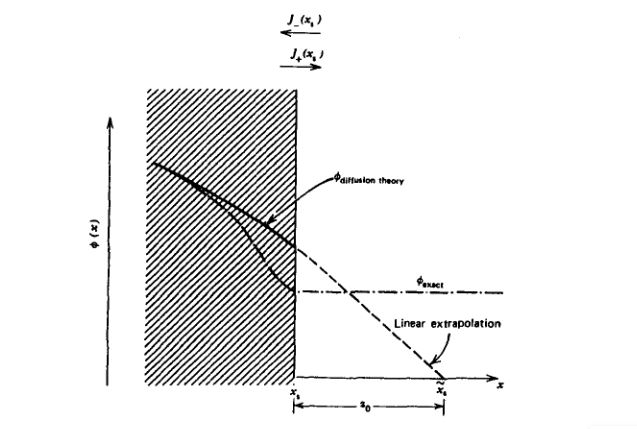
\includegraphics{Fluks.JPG}
    \caption{Prikaz slike spreminjanja fluksa v odvisnosti od razdalje v snovi in vakumu}
    \label{fig:my_label}
\end{figure}
Ta relacija nam v resnici poda, da mora biti odvod fluksa od razdalje enak konstanti, pri čemer lahko z linearnim približkom ugotovimo, da bo fluks enak nič takrat, ko je 
\begin{equation}
    \tilde{x}=x_0+2D
\end{equation}
S tem razlogom pa večkrat v transportni enačbi navajamo, da je robni pogoj v resnici enak
\begin{equation}
    \psi(\tilde{x})=0,
\end{equation}
kjer je $\tilde{x}$ navedena kot referenčna meja.

Če bi naš problem reševali numerično s pomočjo simulacij, bi v resnici ugotovili, da je razdalja pri kateri fluks pade na ničelno vrednost enaka kar $\tilde{x}=x_0+z_0$, kjer je $z_0$ numerično določena konstanta $z_0=0.7104\lambda_{tr}$, kjer je $\lambda_{tr}$ definirana kot prosta pot trasportnega pojava\footnote{$\lambda_{tr}=(\sum_{tr})^{-1}=(\sum_i-\mu_0\sum_s)^{-1}$. $\sum_{tr}$ pa je definira kot transportni sipalni presek, sestavljen pa je iz makroskopsega preseka za transport in sipanje. $\mu_0$ pa prestavlja kosinus povprečnega sipalni kota. Tako nam $\lambda_{tr}$ pove, kako močno je sipanje proti transportu skozi snov}, za katero vemo, da je odvisna od difuzijske konstante kot $D=\frac{\lambda_{tr}}{3}$.\\


V resici je izračun za referenčno dolžino bolj zakompliciran in bi ga lahko opisali z večimi parametri, vendar je to le redkokdaj potrebno. Višje rede aproksimacij v resici vzamemo le takrat, ko se fluks na skali proste poti nevtronov, močneje spreminja s kotom, saj bi tako morali pozabiti na linearno aproksimacijo odvisosti fluksa od kota, ampak bi potrebovali tudi višje rede. S tem pa smo si prišli tudi v protislovje, saj smo si pred začetkom poglavja zatrdili, da se ne smemo nahajati blizu roba, da lahko napravimo to aproksimacijo. V praksi pa se izkaže, da nam robni pogoji dajo primeren fluks le ob sredici reaktorja in sicer nekaj prosti poti stran od njegovega roba. Zato je izpeljava vseh teh enačb uporabna in kljub protislovni predpostavki smisela. \cite{Uvod}

\section{Homogen končni reaktor-problem robni pogojev v vakumu}
Sedaj pa bomo poskusili aproksimirati naše robne pogoje tudi v praksi. Za to si bomo vzeli primer homogenega končnega reaktorja, ki v okolici nima nobenega drugega izvora, hkrati pa so njegovi robni pogoji simetrični in tako neodvisni od kota. Sam reaktor pa je zaradi homogeosti neodvisen od prostora, v katerem ga obravnavamo. 
Za začetek vzemimo našo transportno enačbo s temi pogoji, da velja
\begin{equation}
-D_{g} \nabla^{2} \phi_{g}(\boldsymbol{r})+\Sigma_{\mathrm{i}} \phi_{g}(\boldsymbol{r})=\sum_{h-1 \atop h \neq g}^{G} \Sigma_{g \leftarrow h} \phi_{h}(\boldsymbol{r})+\frac{\chi_{g}}{K_{\mathrm{eff}}} \sum_{h=1}^{G} \nu \Sigma_{\mathrm{f} h} \phi_{h}(\boldsymbol{r})
\label{homogen_1}
\end{equation}
kjer $G$ predstavlja število energijski skupin, $\sum_{h-1 \atop h \neq g}$ predstalja mskroskopski presek za sipanje skupine $h$ na skupini $g$, $\chi_{g}$ je fisijski spekter skupine $g$, $K_{eff}$ izkoristek naše fizije, $\nu \Sigma_{\mathrm{f} h}$ pa predstavlja produkt makroskopskega fizisjeka preseka s številom nevtronov v skupini $h$. Izraz deluje precej zakompliciran, vendar nam v resici pove, da je torej spreminjanje fluksa odvisno od samega fluksa nevtronov pri poziciji $\vec{r}$ (2 člen na levi strani), števila izvorov z določeno energijo (1 člen na desni strani) in fisije produktov izvorov med seboj (2. člen na desni strani). Sam fluks pa bi lahko faktorizirali na odvisost od razdalje in energije $\psi_g(\vec{r})=\psi(\vec{r})\phi_g$ in z vstavljanje tega približka v našo enačbo \eqref{homogen_1} sledi, da je
\begin{equation}
-\frac{\nabla^{2} \psi(\boldsymbol{r})}{\psi(\boldsymbol{r})}=-\frac{\Sigma_{\mathrm{r} g}}{D_{g}}+\frac{1}{D_{g} \varphi_{g}}\left\{\sum_{h-1 \atop h \neq g}^{G} \Sigma_{g \leftarrow h} \varphi_{h}+\frac{\chi_{g}}{K_{\mathrm{eff}}} \sum_{h=1}^{G} \nu \Sigma_{\mathrm{fh}} \varphi_{h}\right\}
\end{equation}
S tem smo sedaj razdelili enačbo na del, ki je zgolj odvisen od pozicije in na del, ki je odvisen zgolj od energije. Da pa sta si obe funkciji za različne vredosti energije in pozicije enaki, pa mora veljati, da sta obe strani enačbe enaki neki konstanti $B^2$, ki jo bomo imenovali kot \textit{bulking of reactor}. S tem dobimo dve med seboj neodvisni enačbi oblike 
\begin{equation}
    \nabla^{2} \psi(\boldsymbol{r})+B^{2} \psi(\boldsymbol{r})=0 \qquad \left[D_{g} B^{2}+\Sigma_{\mathrm{r} g}\right] \varphi_{g}=\sum_{h-1 \atop h \neq g}^{G} \Sigma_{g \leftarrow h} \varphi_{h}+\frac{\chi_{g}}{K_{\mathrm{eff}}} \sum_{h=1}^{G} \nu \Sigma_{\mathrm{f} h} \varphi_{h}
\end{equation}

Takoj opazimo, da je prva enačba v resnici Laplaceva enačba, ki jo bomo rešili s pomočjo robnih pogojev, ki smo ji definirali v poglavju \ref{Robni med dvema}.
\begin{equation}
    \psi(\vec{r})=0 \qquad \nabla\psi(\vec{r})N(\vec{r})=0.
\end{equation}
Da pa bi dobili kakšna je odvisnost od energije, pa bi potrebovali vedeti, kako je porazdeljena energija sistema. Nas pa bo bolj zanimala porazdelitev fluksa po prostoru.
\subsection{Odvisnost fluksa od razdalje}
Kot smo ugotovili, bomo morali reševati Laplacevo enačbo z danimi začetnimi pogoji. Same začetne pogoje pa lahko interpretiramo na več načinov. Glavni razlog v tem pa se skriva, da lahko simetrijo problema $\nabla \psi=0$ obravnavamo v več različni koordinatnih sistemih. 
\subsubsection{Kartezični koordinatni sistem}
V primeru kartezičnega kooridnatnega sistema se nam rešitev Laplaceve enačbe privede v obliko
\begin{equation}
    \nabla^{2} \psi=\frac{\partial^{2} \psi}{\partial x^{2}}+\frac{\partial^{2} \psi}{\partial y^{2}}+\frac{\partial^{2} \psi}{\partial z^{2}} \rightarrow \psi(x, y, z)=C \sin \frac{\pi x}{L_{x}} \sin \frac{\pi y}{L_{y}} \sin \frac{\pi z}{L_{z}}
\end{equation}
kjer so $L_x, L_y, L_z$ dimenzije homogenega reaktorja, za katere velja $0<x,y,z<L_x,L_y,L_z$. Ker pa obravnavamo robni pogoj, vemo, da bo fluks na površini naše domene enak 0. Posledično sledi, ker konstanta $C$ ni ničelna, da je
\begin{equation}
B^{2}=\left(\frac{\pi}{L_{x}}\right)^{2}+\left(\frac{\pi}{L_{y}}\right)^{2}+\left(\frac{\pi}{L_{z}}\right)^{2}.
\end{equation}
\subsubsection{Sferični koordinatni sistem}
V tem primeru se Laplacev operator malce bolj zakomplicira in tako dobimo enačbo
\begin{equation}
\nabla^{2} \psi=\frac{1}{r^{2} \sin \theta}\left[\sin \theta \frac{\partial}{\partial r}\left(r^{2} \frac{\partial \psi}{\partial r}\right)+\frac{\partial}{\partial \theta}\left(\sin \theta \frac{\partial \psi}{\partial \theta}\right)+\frac{1}{\sin \theta} \frac{\partial^{2} \psi}{\partial \epsilon^{2}}\right]
\end{equation}
Vendar ker vemo, da je naš izvor homogen, lako kotno odvisnos reaktorja zaemarimo in tako ob robnemu pogoju ničelnega fluksa sledi, da je 
\begin{equation}
    \psi(\vec{r})=\frac{C}{r}\sin\left(\frac{\pi r}{R}\right) \rightarrow B^2=\left(\frac{\pi}{R}\right)^2
\end{equation}
kjer je R dimenzija našega reakorja. 
\subsubsection{Cilindrični koordinatni sistem}
V primeru cilindričnega kooridnatnega sistema pa bi dobili Laplacev operator v obliki
\begin{equation}
\nabla^{2} \psi=\frac{1}{\rho}\left[\frac{\partial}{\partial \rho}\left(\rho \frac{\partial \psi}{\partial \rho}\right)+\frac{1}{\rho} \frac{\partial^{2} \psi}{\partial \epsilon^{2}}+\rho \frac{\partial^{2} \psi}{\partial z^{2}}\right]
\end{equation}
Glava rešitev problema reaktorja z radijem $R$ in višino $h$ pa se tako glasi
\begin{equation}
\psi(\rho, z)=C J_{0}\left(\frac{2.405 \rho}{R}\right) \sin \frac{\pi z}{L_{z}} \rightarrow 
B^{2}=\left(\frac{2.405}{R}\right)^{2}+\left(\frac{\pi}{L_{z}}\right)^{2}
\end{equation}

kjer $J_0(x)$ predstavlja ničelno Besslovo funkcijo, za katero velja, da je $J_0(2.405)=0$


\section{Enodimenzionalni heterogen reaktor}
Sedaj pa si poglejmo nalogo, ko nevtronski fluks prehaja skozi več plasti. Naša predpostavka pa bo, da lastnosti reaktorja odvisne zgolj od ene smeri in sicer $x$. S tem se nam naša transportna enačba, ki smo jo definirali v prejšnjem poglavju prepiše v obliko
\begin{equation}
\begin{aligned}
-\frac{d}{d x} D_{g}(x) \frac{d \phi_{g}}{d x}+\Sigma_{\mathrm{rg}}(x) \phi_{g}(x)
=\sum_{h=1 \atop h \neq g}^{G} \Sigma_{g \vdash h}(x) \phi_{h}(x)+\frac{\chi_{g}(x)}{K_{\mathrm{eff}}} \sum_{h=1}^{G} \nu \Sigma_{f h(x) \phi_{h}(x)}
\label{homogen_2}
\end{aligned}
\end{equation}
Naš robni pogoj pa lahko definiramo na dva načina. Lahko vzamemo osnovni robni pogoj, da velja $\psi_g(x)=0$, druga možnost pa je, da si pogledamo, kaj se dogaja z pogojem albeda \eqref{Albedo}, ki ga zapišemo v malo drugačni obliki, saj upoštevamo, da je v tem primeru difuzijska konstanta odvisna od lokacije
\begin{equation}
\mp D_{g}(x) \frac{d \phi_{g}}{d x}+\frac{1}{2} \frac{1-\beta(x)}{1+\beta(x)} \phi_{g}(x)=0
\label{Homogen slab}
\end{equation}
kjer $\beta$ predstavlja albedo, predznak pa je odvisen od tega, kateri robin pogoj vzamemo. V primeru levega robnega pogoja $x=x_{\frac{i}{2}}$ velja - medtem ko za desni robni pogoj $x=x_{\frac{1}{2}+i}$ velja +. \footnote{$\beta(\vec{r})=\frac{J^-_g(\vec{r})}{J^+_g(\vec{r})}$ ali albedo nam v resici pove, kako močan je pritok in kako močan je odtok nevtronov skozi neko ploščo. Pri poglavju \ref{Robni med dvema} ga nismo definirali zato, ker smo predpostavili, da ni pritokov in odtokov elektronov in je bil zati $\beta=0$.}\\

Za vsako plast pa predpostavimo, da je homogena in da ima svoje lastnosti. Tako lahko reaktor razdelimo na $I$ delov in vsaki regiji pripišemo enačbo \eqref{Homogen slab} v obliki
\begin{equation}
-D_{g, i} \frac{d^{2} \phi_{g}}{d x^{2}}+\Sigma_{\mathrm{r} g, i} \phi_{g}(x)=Q_{g}^{\circ}(x)=\sum_{h=1 \atop h \neq g}^{G} \Sigma_{g \leftarrow h, i} \phi_{h}(x)+\frac{\chi_{g, i}}{K_{\text {eff }}} \sum_{h=1}^{G} \nu \Sigma_{\mathrm{f} h, i} \phi_{h}(x) 
\end{equation}

v primeru, ko je $x_{i-\frac{1}{2}-}<x<x_{\frac{1}{2}+i}$.


Da bi lahko dobili analitično rešiev našega problema, pa moramo enačbo prepisati v obliko, ki bi jo znali rešiti. Zato pa bi bil najbolj ustrezen matrični zapis naših količin, da velja 
\begin{equation}
\begin{gathered}
\frac{d^{2}}{d x^{2}} \Phi(x)+\mathbb{F}_{i} \Phi(x)=0 \quad \text { if } x_{i-1 / 2}<x<x_{i+1 / 2} \\
\Phi(x)=\left(\begin{array}{c}
\phi_{1}(x) \\
\vdots \\
\phi_{G}(x)
\end{array}\right) \quad \text { i } \quad \mathbb{F}_{i}=\left(\begin{array}{cccc}
f_{11, i} & f_{12, i} & \ldots & f_{1 G, i} \\
f_{21,8} & f_{22, i} & \ldots & f_{2 G, i} \\
\vdots & \vdots & \ddots & \vdots \\
f_{G 1,2} & f_{G 2, i} & \ldots & f_{G G, i}
\end{array}\right)
\end{gathered}
\end{equation}
kjer so koeficienti komponet matrike $\mathbb{F}_{i}$ enaki 
\begin{equation}
f_{g h, i}=\frac{1}{D_{g, i}}\left[-\Sigma_{\mathrm{r} g, i} \delta_{g h}+\Sigma_{g \leftarrow h, i}\left(1-\delta_{g h}\right)+\frac{\chi_{g, i}}{K_{\mathrm{eff}}} \nu \Sigma_{\mathrm{f} h, i}\right]
\end{equation}

Tako smo naš problem privedli do reševanja matrične forme in iskanja lastnih vrednosti. V našem primeru si bomo preuredili prolem tako, da velja 
\begin{equation}
\frac{d^{2}}{d x^{2}} \Psi(x)+\operatorname{diag}\left(\lambda_{\ell, i}\right) \Psi(x)=0 \quad \text { if } x_{i-1 / 2}<x<x_{i+1 / 2},
\label{matrični}
\end{equation}
kjer so $\lambda_{l,i}$ lastne vrednosti sistema
\begin{equation}
\mathbb{F}_{i} \mathbb{T}_{t}=\mathbb{T}_{i} \operatorname{diag}\left(\lambda_{\ell, i}\right) \qquad \mathbb{T}_{t} \text{ predstavlja lastni vektor našega sistema}
\end{equation}
Sam vektor $\psi$ pa definiramo preko enačbe \begin{equation}
\Phi(x)=\mathbb{T}_{i} \Psi(x)=\left(\begin{array}{cccc}
t_{11, i} & t_{12, i} & \ldots & t_{1 G, i} \\
t_{21, i} & t_{22, i} & \ldots & t_{2 G, i} \\
\vdots & \vdots & \ddots & \vdots \\
t_{G 1, i} & t_{G 2, i} & \ldots & t_{G G, i}
\end{array}\right)\left(\begin{array}{c}
\psi_{1}(x) \\
\psi_{2}(x) \\
\vdots \\
\psi_{G}(x)
\end{array}\right),
\label{psi}
\end{equation}

V takem matričnem sistemu, ki ga poda enačba \eqref{matrični} pa prepoznamo analitične rešitve oblike
\begin{equation}
\psi_{g}(x)= \begin{cases}A_{g, i} \cos \left(\sqrt{\lambda_{g, i}} x\right)+B_{g, i} \sin \left(\sqrt{\lambda_{g, i}} x\right) & \text { if } \lambda_{g, i} \geq 0 ; \\ C_{g, i} \cosh \left(\sqrt{-\lambda_{g, i}} x\right)+E_{g, i} \sinh \left(\sqrt{-\lambda_{g, i}} x\right) & \text { otherwise }\end{cases}
\end{equation}

Tako bomo dobili, da je vrednost fluksa pri določeni energiji iz enačbe \eqref{psi}
enaka kar 
\begin{equation}
    \phi_g(x)=\sum_{h=1}^G t_{gh,t}\psi_h(x)
\end{equation}
Kot zadnji korak pa moramo upoštevati še robne pogoje med dvema različnima snovema. Že prej smo izpeljali, da mora biti fluks na robu zvezen in zvezno odvedljiv, zato vemo, da bo tudi v tem primeru veljalo, da je za vsako mejo 
\begin{equation}
\begin{gathered}
\phi_{g}\left(x_{i\pm1 / 2}^{-}\right)=\phi_{g}\left(x_{i\pm1 / 2}^{+}\right) \\
D_{g, i-1} \phi_{g}^{\prime}\left(x_{i\pm1 / 2}^{-}\right)=D_{g, i} \phi_{g}^{\prime}\left(x_{i\pm1 / 2}^{+}\right)
\end{gathered}
\end{equation}

S tema dvema robnima pogojema pa bomo lahko tudi izračunalo, kolikšne so vrednosti konstant $A_{g, i},B_{g, i} ,C_{g, i} ,D_{g, i} $ za vsak sloj našega reaktorja. \\

S tem smo definirali, kako bi problem reševali v primeru, ko bi imeli končno mnogo slojev, za vajo pa bomo rešili problem dveh slojev, v katerega bomo poskusili vpeljati smiselne robne pogoje.
\subsection{Robni problem dveh slojev z matričnim zapisom}
Že v začetku obravnave dveh slojev se naša enačba \eqref{homogen_2} poenostavi v obliko
\begin{equation}
\begin{aligned}
-D_{i} \frac{d^{2} \phi}{d x^{2}}+\Sigma_{\mathrm{r}, i} \phi(x)=& \frac{1}{K_{\mathrm{eff}}} \nu \Sigma_{\mathrm{f}, i} \phi(x)  \quad \text { if } x_{i-1 / 2}<x<x_{i+1 / 2}
\end{aligned}
\end{equation}
Takoj lahko opazimo, da je enačba podobna obliki nihajne enačbe in bodo zato rešitve zgolj kombinacije funkcij $\sin$ in $\cos$. Tako lahko rešitev v odvisnosti od konstant $\kappa_i$ zapišemo kot\footnote{Izpeljave, zakaj pridejo ravno kotne funckije sinusov in kosinusov v tem seminarju ne bomo naredili, saj se bomo osredotočali zgolj na uvedbo robni pogojev v naš problem}
\begin{equation}
\phi(x)= \begin{cases}A_{11} \cos \left(\kappa_{1} x\right)+A_{21} \sin \left(\kappa_{1} x\right) & \text { if } 0 \leq x \leq \frac{1}{2} \\ A_{12} \cos \left(\kappa_{2} x\right)+A_{22} \sin \left(\kappa_{2} x\right) & \text { if } \frac{1}{2} \leq x \leq 1\end{cases}
\end{equation}
Sedaj, ko imamo zapisane rešitve fluksa za prvo in drugo plast pa moramo ugotoviti, kolikšne so vrednosti danih parametrov. To pa lahko storimo z vpogledom v robne pogoje našega problema. \\

Iz ničelnega pogoja za fluks takoj sledi, da mora veljati, da je
\begin{equation}
    \psi(0)=A_{11}=0.
\end{equation}
Drugi pogoj nam bo podal, da mora biti na robu med dvema ploskvama $x=\frac{1}{2}$ fluks in odvod fluksa preko enačbe \eqref{robni_2} zvezen. Tako dobimo, z upoštevanjem $A_{11}=0$, naslednjo zvezo
\begin{equation}
\begin{aligned}
&A_{21} \sin \left(\frac{\kappa_{1}}{2}\right)=A_{12} \cos \left(\frac{\kappa_{2}}{2}\right)+A_{22} \sin \left(\frac{\kappa_{2}}{2}\right) \\
&A_{21} \kappa_{1} D_{1} \cos \left(\frac{\kappa_{1}}{2}\right)=-A_{12} \kappa_{2} D_{2} \sin \left(\frac{\kappa_{2}}{2}\right)+A_{22} \kappa_{2} D_{2} \cos \left(\frac{\kappa_{2}}{2}\right)
\end{aligned}
\end{equation}

Če pa upoštevamo še zvezo, da je fluks na desnem robu naše druge plošče ($x=1$) ničeln bo tako veljalo, da je
\begin{equation}
A_{22}=A_{12} \tan \left(\kappa_{2}\right)
\end{equation}
Z preurejanjem enačb tako lahko dobimo rešitev, ki je odvisna zgolj od koeficientov $A_{21}$ in $A_{12}$.
\begin{equation}
\textbf{M}\textbf{A}=\left(\begin{array}{cc}
\sin \left(\frac{\kappa_{1}}{2}\right) & -\frac{1}{\cos \left(\kappa_{2}\right)} \cos \left(\frac{\kappa_{2}}{2}\right) \\
\kappa_{1} D_{1} \cos \left(\frac{\kappa_{1}}{2}\right) & -\frac{\kappa_{2} D_{2}}{\cos \left(\kappa_{2}\right)} \sin \left(\frac{\kappa_{2}}{2}\right)
\end{array}\right)\left(\begin{array}{l}
A_{21} \\
A_{12}
\end{array}\right)=\left(\begin{array}{l}
0 \\
0
\end{array}\right)
\end{equation}
Tak sistem pa ima e
trivialno rešitev le takrat, ko je determinata matrike $\textbf{M}$ enaka 0. S upoštevajem tega pogoja pa dobimo nelinarno relacijo med $\kappa_1$ in $\kappa_2$. 
\begin{equation}
\tan \left(\frac{\kappa_{1}}{2}\right) \tan \left(\frac{\kappa_{2}}{2}\right)=\frac{\kappa_{1} D_{1}}{\kappa_{2} D_{2}} \quad \kappa_{1}=\sqrt{\frac{\nu \Sigma_{\mathrm{f}, 1}-K_{\mathrm{eff}} \Sigma_{\mathrm{r}, 1}}{K_{\mathrm{eff}} D_{1}}} \text { in} \kappa_{2}=\sqrt{\frac{\nu \Sigma_{\mathrm{f}, 2}-K_{\mathrm{eff}} \Sigma_{\mathrm{r}, 2}}{K_{\text {eff }} D_{2}}}
\end{equation}
kjer smo za ugotovitve vrednosti $\kappa_1$ vzeli kar našo začetno enačbo transportnega pojava. Vidimo, da sama neliearna zveza med vrednostmi $\kappa$ ni analitično rešljiva, da pa se jo rešiti grafično ali numerično (primer bisekcija) in tako prilagoditi parametra, da rešitev obstaja. \\

Če sedaj znane vrednosti konstant vstavimo v našo rešitev za fluks, dobimo 
\begin{equation}
\phi(x)= \begin{cases}A_{21} \sin \left(\kappa_{1} x\right) & \text { if } 0 \leq x \leq \frac{1}{2} \\ A_{21} \frac{\sin \left(\frac{\kappa_{1}}{2}\right)}{\cos \left(\frac{\kappa_{2}}{2}\right)} \cos \left[\kappa_{2}(1-x)\right] & \text { if } \frac{1}{2} \leq x \leq 1\end{cases}.
\end{equation}
Razvidno pa je, da se bo torej nevtronski fluks odzival na spremembo konstate $A_{21}$. Za njeno točno vrednost pa bi morali uporabiti še začetne pogoje našega problema in tako ugotoviti, točno funkcijo fluksa v odvisnosti od razdalje. \cite{Homogeni}

\newpage

\section{Zaključek}
Vidimo, da so v resnici robni pogoji naših enačb zelo pomembni za izbiro rešitev, ki pripadajo problemu. Kot smo opazili, pa se pri reševanju transportne enačbe vedno zanašamo na to, da je fluks zvezen in zvezno odvedljiv na robu našega problema. Ta rešitev se tudi v naravi zdi smiselna, saj se nevtroni gibljejo s pomočjo Browovega gibanja, ki pa je kljub naključnosti zvezno (delec ne preskoči med dvema legama). 

Vredno pa je bilo tudi opaziti, da lahko v primeru veči robnih plasti problem obravavamo v matrični obliki. Glavni razlog za to pa je, da nam matematični formalizem, ki se skriva za matričnim zapisom poda lažje reševanje problema preko lastnih vrednosti, kot pa da bi morali reševati sistem sklopljenih diferencialnih enačb. 

\printbibliography


                                                                                                                                                                                                                                                                                                                                                                                                                                                                                                                                                                                                                                                                                                                                                                                                                                                                                                                                                                                                                                                                                                                                                                                                                                                                                                                                                                                                                                                                                                                                                                                                                 
\end{document}
